\documentclass[border=4pt]{standalone}
\usepackage{pgfplots}
\pgfplotsset{compat=1.18}

\begin{document}
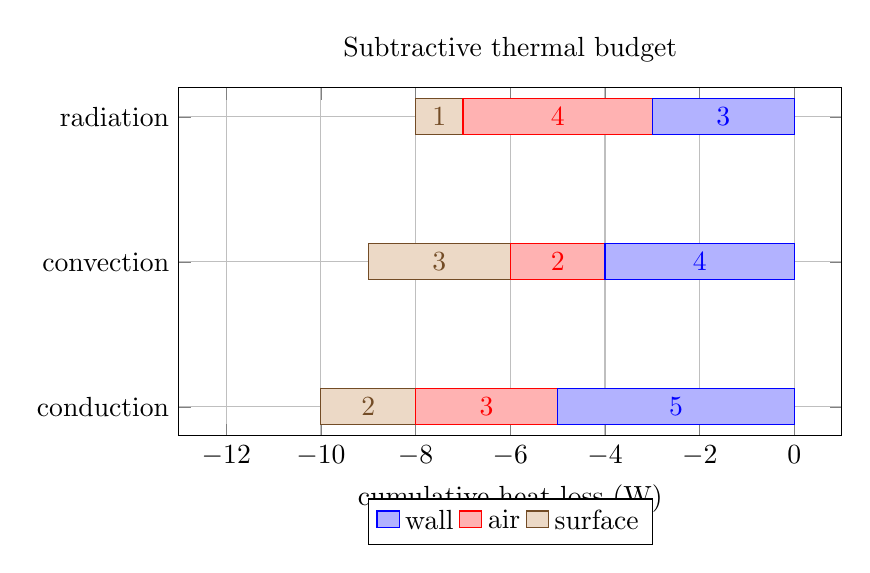
\begin{tikzpicture}
  \begin{axis}[
    xbar stacked=minus,
    stack negative=on previous,
    width=10cm,
    height=6cm,
    bar width=13pt,
    xmin=-13,
    xmax=1,
    ytick={1,2,3},
    yticklabels={conduction,convection,radiation},
    xlabel={cumulative heat loss (W)},
    title={Subtractive thermal budget},
    grid=major,
    nodes near coords,
    legend style={at={(0.5,-0.18)},anchor=north,legend columns=-1}
  ]
    \addplot coordinates {(5,1) (4,2) (3,3)};
    \addplot coordinates {(3,1) (2,2) (4,3)};
    \addplot coordinates {(2,1) (3,2) (1,3)};
    \legend{wall,air,surface}
  \end{axis}
\end{tikzpicture}
\end{document}
